%% ============================================================
%% 分片 28：原文第 10 节「The Bogomolny Equations And The Space Of Hecke Modifications」（原文 glshort.tex 起于第 8120 行）
%% 由 tools/harvmac2tex.py 从 arXiv 源码（hep-th/0604151v3）自动生成。
%% 只译英文散文；公式、编号、\label、\cite 一律不改。
%% ============================================================

\subsection{Kahler Structure And The Moment Map}

\label{sec:kahstr}

Our next goal is to exhibit ${\EUZ}({}^L\negthinspace
w_1,\dots,{}^L\negthinspace w_n)$ as a Kahler manifold, with a
complex structure that agrees with the appropriate moduli space of
Hecke modifications, as described in section 第~\ref{sec:thooftheckeop}~节. This
analysis will make many things clearer.  It will give a new
motivation for the choice of boundary conditions that we used in
defining ${\EUZ}$; it will give a more precise framework for
understanding the relation between 't Hooft and Hecke operators;
and it will make more transparent the properties of the
singularities of the space of Hecke modifications.

\begin{figure}[htbp]
\centering
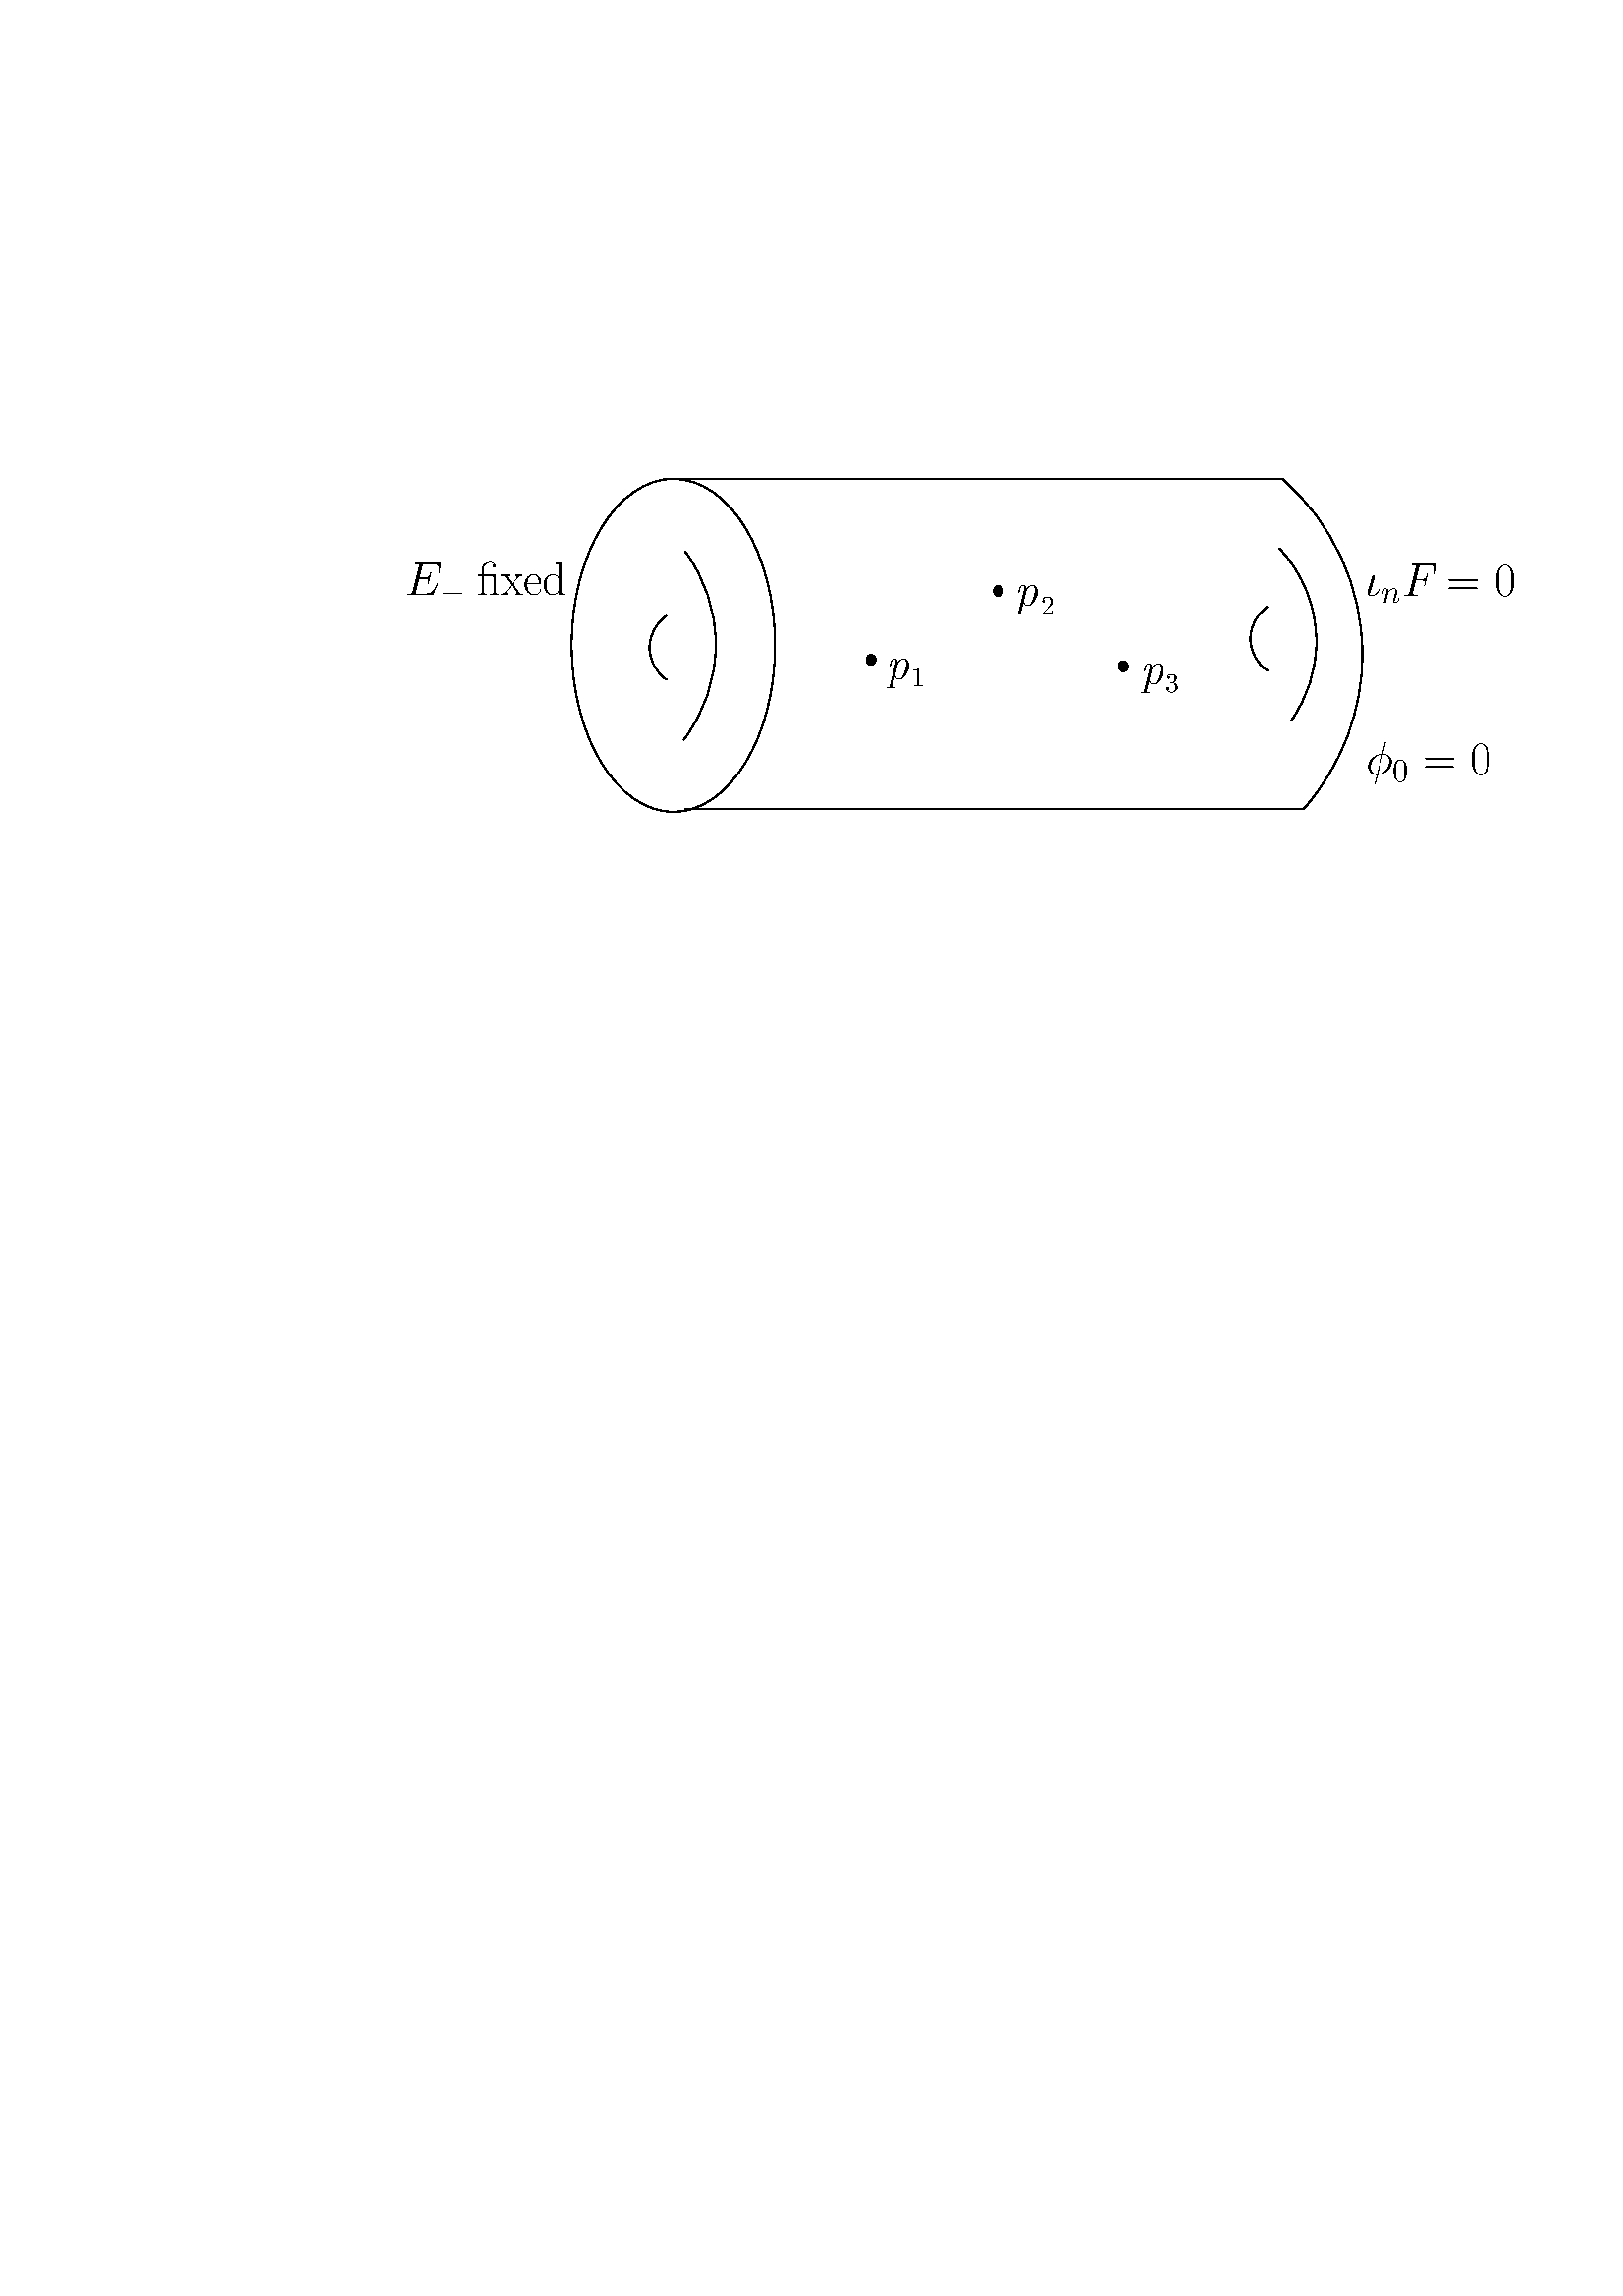
\includegraphics[width=0.75\linewidth]{figures/gla7-5.png}
\caption{Comparing 't Hooft and Hecke operators on a three-manifold $W=I\times C$. On the left, a connection $A$ and bundle $E_-$ are specified, and the gauge transformations are required to be trivial. On the right, one sets $\phi_0=0$ and solves for $E_+$.（原文 Fig.~16）}
\label{fig:xutampo}
\end{figure}

As in the introduction to section 第~\ref{sec:thooftheckeop}~节, we take the
metric of the three-manifold $W=I\times C$ to be of the form
$ds^2=h|dz|^2+dy^2$, where $z=x^2+ix^3$ is a local complex
coordinate on $C$ and $y$ parametrizes $I$. We consider the
Bogomolny equations $F=\star D\phi_0$, where $F$ is the curvature
of a connection $A$ on a $G$-bundle $E$.  At the left end of $W$,
we specify a flat $G$-bundle $E_-$, and divide only by gauge
transformations that equal 1 on the boundary; at the right end, we
require $\phi_0=0$ with and divide by all gauge transformations.

 We expand the
connection as $A=A_z dz+A_{\bar z}d\bar z+A_ydy=A_2dx^2+A_3
dx^3+A_ydy$. By rewriting \eqref{eq:noffo}\ and \eqref{eq:jungol}, the Bogomolny
equations in these coordinates can be written as a complex
equation % 式 (10.14)
\setcounter{equation}{13}
\begin{equation}\label{eq:mirot}
\left[D_y-i\phi_0, D_{\bar z}\right]=0
\end{equation}
 and a
real equation % 式 (10.15)
\setcounter{equation}{14}
\begin{equation}\label{eq:irot}
F_{23}=hD_y\phi_0.
\end{equation}

On the space $\EUC$ of fields $(A,\phi_0)$, we introduce a complex
structure ${\cal I}$ in which the complex coordinates are $A_{\bar
z}$ and $B=A_y-i\phi_0$.  The rationale for this choice is that
the complex equation in \eqref{eq:mirot}\ is holomorphic in this complex
structure. Furthermore, we endow $\EUC$ with the symplectic
structure % 式 (10.16)
\setcounter{equation}{15}
\begin{equation}\label{eq:uryt}
\omega=\int_{W}\Tr\Bigl(\delta A_2\wedge
\delta A_3-h\,\delta A_1\wedge \delta\phi_0\Bigr) dx^2\,dx^3\,dy.
\end{equation}

The complex structure ${\cal I}$ and symplectic structure $\omega$
combine to a Kahler structure, the Kahler metric being
% 式 (10.17)
\setcounter{equation}{16}
\begin{equation}\label{eq:ryt}
-\int_W\Tr\Bigl( \delta A_2\otimes \delta A_2+\delta
A_3\otimes \delta A_3+h\,\delta A_y\otimes \delta A_y+h\,\delta
\phi_0\otimes \delta \phi_0\Bigr)dx^2\,dx^3\,dy.
\end{equation}

Now we want to find the moment map $\mu$ for the action of the
gauge group.  As usual, the moment map $\mu(v)$ for a symplectic
vector field $v$ is characterized by
% 式 (10.18)
\setcounter{equation}{17}
\begin{equation}\label{eq:charby}
d\mu(v)=\iota_v\omega,
\end{equation}
 where $\iota_v$ is the
operation of ``contracting with $v$.'' For the vector field
characterized by the infinitesimal gauge transformation that acts
by $\delta A=-D\epsilon$ and $\delta\phi_0 =[\epsilon,\phi_0]$,
with $\epsilon\in \Omega^0(C,{\rm ad}(E))$, we find the moment map
to be % 式 (10.19)
\setcounter{equation}{18}
\begin{equation}\label{eq:prigo}
\mu(\epsilon)=\int_W\Tr\left(\epsilon(
\,F_{23}-hD_y\phi_0)\right)dx^2\,dx^3\,dy+ \int_{\partial
W}\,\Tr\,(\epsilon\phi_0) \,h\,dx^2\,dx^3.
\end{equation}
 The calculation is
similar to that in deriving eqn. \eqref{eq:joget}, except that a boundary
term appears in integration by parts.

In the presence of 't Hooft operators at points $p_i\in W$, we
modify the definitions slightly.  $A$ and $\phi_0$ are required to
have prescribed singularities near  $p_i$.  And $\epsilon$ is
constrained near $p_i$ to generate a gauge transformation that
leaves fixed the chosen singularity. Our formulas for the moment
map remain valid in this situation.

We want to interpret the real Bogomolny equation \eqref{eq:irot}\ in terms
of the vanishing of the moment map.  In fact, for $\mu(\epsilon)$
to vanish does give us \eqref{eq:irot}\ together with another condition:
$\Tr\,\epsilon\phi_0$ must vanish on the boundary.  On any given
boundary component $C_\pm$ of $W$, there are two simple ways to
ensure that $\Tr\,\epsilon\phi_0=0$.  We can set $\epsilon=0$ on
the boundary, in other words we can allow only gauge
transformations that are trivial on this boundary component. Or we
can set $\phi_0=0$.  To define the moduli space ${\EUZ}$, we have
used (\xutampo) one of these boundary conditions on $C_-$, and the
other on $C_+$.  Thus we have a new rationale for our boundary
conditions: they are the simplest ones that allow us to interpret
the Bogomolny equations in terms of a holomorphic equation
together with the vanishing of the moment map.

Now we can invoke the usual correspondence between symplectic
quotients and complex quotients.  Let ${\EUC}_0$ be the subspace
of $\EUC$ characterized by vanishing of the holomorphic Bogomolny
equation \eqref{eq:mirot}.  The moduli space ${\EUZ}$ is defined by setting
$\mu $ to zero and dividing by the group $\cal G$ of $G$-valued
gauge transformations.  We can compare it to
${\EUZ}'={\EUC}_0/{\cal G}_{\Bbb{C}}$, the quotient of ${\EUC}_0$
by the complexified group ${\cal G}_{\Bbb{C}}$ of ${
G}_{\Bbb{C}}$-valued gauge transformations.

Of course, because of the boundary conditions, $\cal G$ is the
group of gauge transformations that are trivial at the left end of
$W$, and likewise ${\cal  G}_{\Bbb{C}}$ is the group of
$G_{\Bbb{C}}$-valued gauge transformations that are trivial at
that end.

 Usually, in comparing a symplectic quotient to the
corresponding complex quotient, one has to worry about possible
unstable and semistable orbits.  In the present case, however,
because the gauge transformations are restricted to be trivial at
one end of $W$, such issues are avoided.  ${\cal G}_{\Bbb{C}}$
acts freely and with closed orbits, so all orbits are stable and
${\EUZ}={\EUZ}'$.

It is straightforward to analyze ${\EUZ}'$.  In fact, we have
essentially done so in section 第~\ref{sec:theck}~节.  For any $y\in I$ away from
the location of an 't Hooft operator, let $E_y=E|_{ \{y\}\times
C}$. The complex Bogomolny equation says that the holomorphic type
of $E_y$ is independent of $y$, as long as one does not cross the
position of an 't Hooft operator.  Moreover, this holomorphic type
is the only ${\cal G}_{\Bbb{C}}$-invariant in an interval without
't Hooft operators.  In jumping across 't Hooft operators, $E_y$
undergoes Hecke modifications. So ${\EUZ}'$ is the space of Hecke
modifications of $E_-$ due to the prescribed singularities.

This comparison of complex and symplectic quotients thus gives a
precise framework for understanding the relationship between 't
Hooft and Hecke operators, which we compared more informally in
section 第~\ref{sec:theck}~节.  In addition, it will enable us to understand
better some properties of the spaces of Hecke modifications that
were described in section 第~\ref{sec:spaceheck}~节 .

\par\medskip{\it Changing the Complex And Symplectic
Structures}

Let us denote the points $p_i$ in $W=I\times C$ at which 't Hooft
operators are inserted as $y_i\times z_i$, with $y_i\in I$ and
$z_i\in C$.  We want to understand the dependence of the moduli
space ${\EUZ}$ on the points $p_i$.

It is convenient to introduce the modified connection
$A'=A-i\phi_0 dy$, the idea being that if we expand
$A'=dz\,A'_z+d\bar z \,A'_{\bar z} +dy\, A'_y$, then $A'{}_y$ and
$A'{}_{\bar z}$ are holomorphic in complex structure ${\cal I}$,
although $A'_z$ is not.  Since $A$ is real,  that is, it takes
values in the real Lie algebra of $G$, $A'_z$ (which equals $A_z$)
is the complex conjugate of $A'_{\bar z}$; of course, $A'_y$ obeys
no reality condition. To describe a holomorphic group action on
the space $\EUC$ of pairs $(A,\phi_0)$, which is the same as the
space of modified connections $A'$, it suffices to describe how
$A'_{\bar z}$ and $A'_y$ transform.  The transformation of $A'_z$
is then determined by the fact that it is the complex conjugate of
$A'_{\bar z}$.

 Consider
$W=I\times C$ as a fiber bundle over $C$, and let $D_I$ be the
group of  diffeomorphisms of $W$ that preserve this fibration.
Such a diffeomorphism, while keeping $z$ fixed, maps $y$ to
$\tilde y(y;z,\bar z)$, where $\tilde y$ agrees with $y$ on the
boundaries of $W$ and $\partial \tilde y/\partial y>0$.  We define
an action of $D_I$ on $\EUC$  by simply saying that $A'_{\bar z}$
and $A'_y$ transform in the natural way, by the ``pullback.''

Note that we cannot transform $A'$ by pullback; for $\beta\in
D_I$, the operation $A'\to \beta^*(A')$ would not preserve the
fact that $A'_z$ and $A'_{\bar z}$ are complex conjugates. Instead
we define $\beta(A')=\beta^*(A')+dz\,\varepsilon$, where
$\varepsilon$ is determined to retain the condition that $A'_z$
and $A'_{\bar z}$ are complex conjugates.

This action of $D_I$ on the space $\EUC$ of pairs $(A,\phi_0)$
preserves the complex structure ${\cal I}$.  It also preserves the
complex Bogomolny equation,  so it preserves the space ${\EUC}_0$
of solutions of that equation.  These statements depend on the
fact that diffeomorphisms in $D_I$ keep $z$ fixed. They therefore
preserve the foliation generated by $\partial/\partial y$ and
$\partial/\partial \bar z$ , and the assertion of flatness along
leaves of this foliation -- which is the content of the complex
Bogomolny equation -- is invariant. In addition, $D_I$ maps the
group ${\cal G}_{\Bbb{C}}$ of $G_{\Bbb{C}}$-valued gauge
transformations of $\EUC$  to itself. So ${\EUZ}$, defined as a
complex manifold by ${\EUZ}={\EUC}_0/{\cal G}_{\Bbb{C}}$, is
invariant under $D_I$.

However, the symplectic form $\omega$ on $\EUC$ is definitely not
$D_I$-invariant, and accordingly neither is the moment map for the
${\cal G}$ action, or the real Bogomolny equation.  So ${\EUZ}$,
understood as the symplectic quotient of ${\EUC}_0$ by the action
of ${\cal G}$, using the symplectic structure $\omega$, is not
invariant under $D_I$.

The conclusion is that the complex structure of ${\EUZ}$ is
$D_I$-invariant, but not its symplectic structure.

Now let us consider 't Hooft operators at points $p_i=y_i\times
z_i$.  The group $D_I$ can slide the $p_i$ up and down in the $y$
direction, in a fashion that is arbitrary except for one
restriction: if two $p_i$ are at the same value of $z$, then their
ordering in the $y$ direction is $D_I$-invariant. The conclusion
is that sliding the points $p_i$ in the $y$ direction, without
letting two points at the same $z$ cross each other, changes the
symplectic structure of $\EUZ$ but not its complex structure.

There is also a reverse version of this.  The definition of the
symplectic structure of $\EUC$ used the area form of $C$, but not
its complex structure.  The same is, therefore, true for the
moment map $\mu$.  So just given the area form of $C$, we can
define the symplectic quotient $\EUC/\negthinspace/{\cal
G}=\mu^{-1}(0)/{\cal G}$. This is an infinite-dimensional
symplectic manifold whose symplectic structure depends only on the
area form of $C$.  Now in general, in a symplectic manifold, a
family of symplectic submanifolds defined by a varying family of
equations has a fixed symplectic structure.  In our application,
the varying family of equations are the complex Bogomolny
equations, which depend on the complex structure of $C$. So as the
complex structure and the positions of the points vary, the
complex structure of ${\EUZ}$ may change, but the symplectic
structure does not.

If 't Hooft operators are inserted at point $p_i=y_i\times z_i\in
I\times C$, then changing the $z_i$ with the $y_i$ fixed, and
without changing whether or not $z_i=z_j$ for a given pair $i,j$,
is equivalent to a special case of changing the complex structure
of $C$.  So changing the $z_i$ in this way changes the complex
structure of ${\EUZ}$ but not its symplectic structure.

\par\medskip{\it Comparison To Holomorphic Results}

We can use these observations to get a new perspective on some
facts that we described in section 第~\ref{sec:spaceheck}~节 .

\begin{figure}[htbp]
\centering
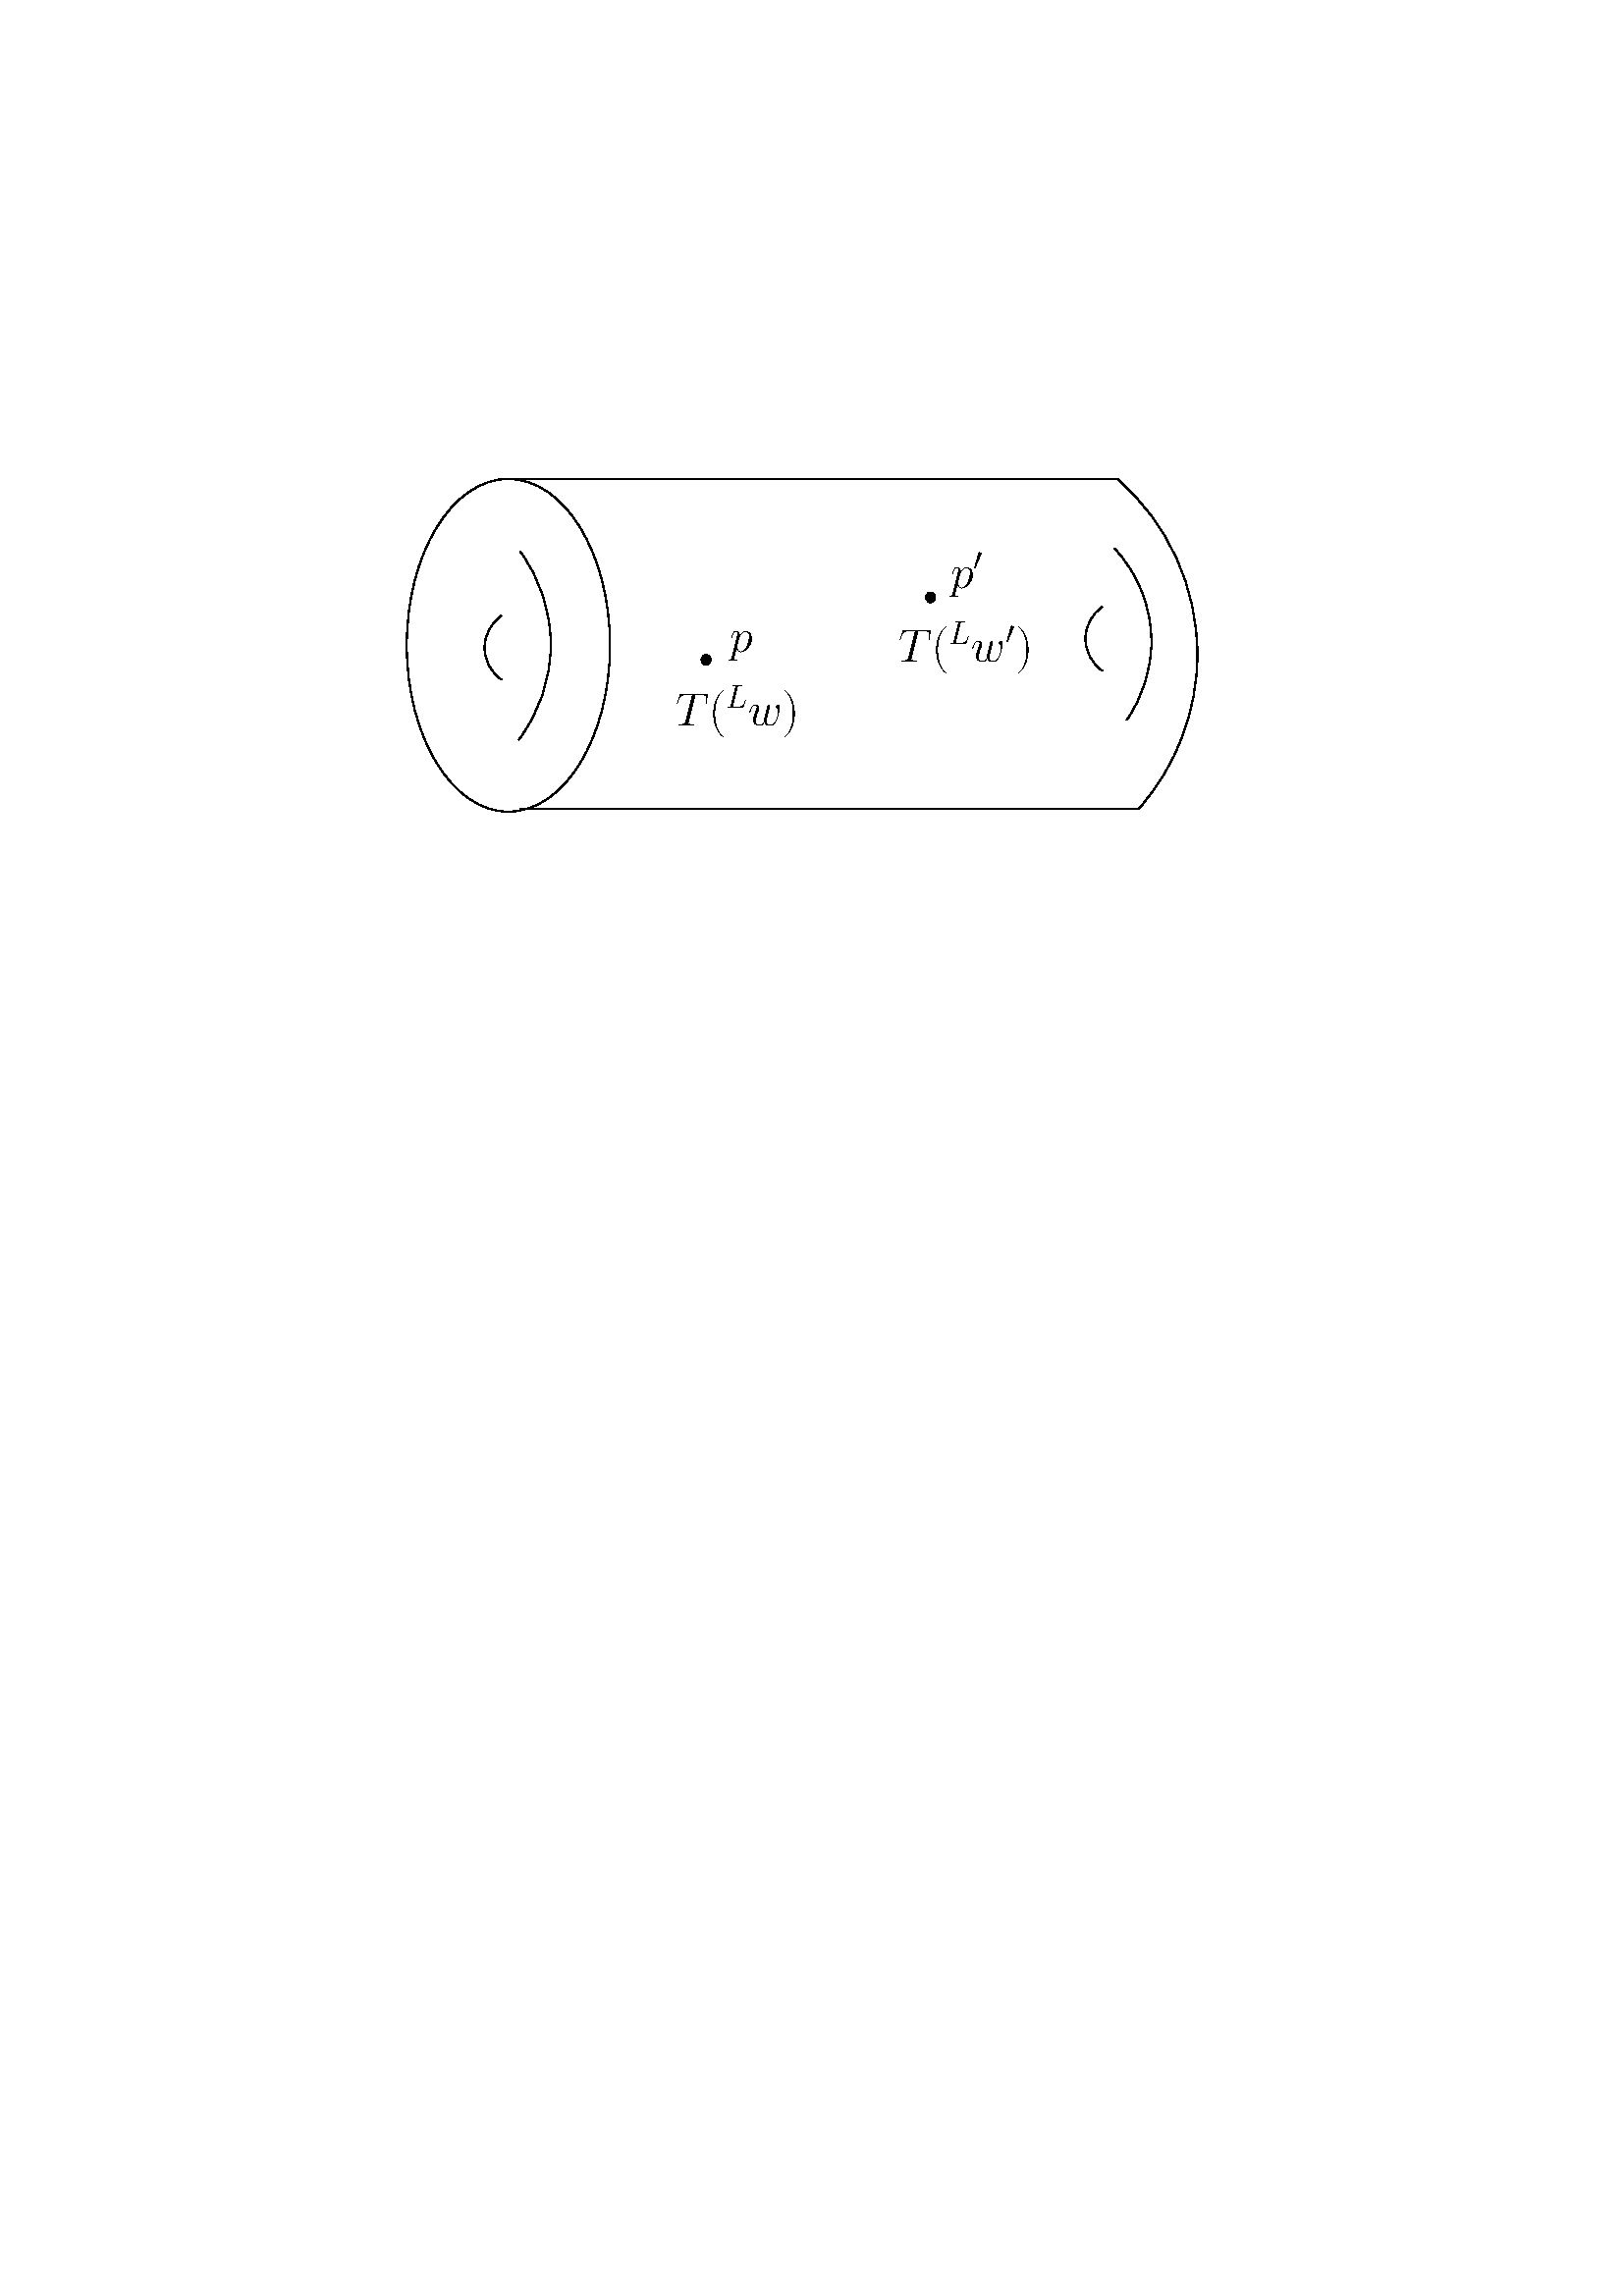
\includegraphics[width=0.75\linewidth]{figures/gla7-6.png}
\caption{Insertion of two 't Hooft operators of weights $^L\negthinspace w$ and $^L\negthinspace w'$ at points $p,p'\in W$.（原文 Fig.~17）}
\label{fig:xtampo}
\end{figure}

Consider $W=I\times C$ with insertion of two 't Hooft operators
$T(^L\negthinspace w,p)$ and $T(^L\negthinspace w',p')$ of the
indicated weights,  inserted
 at $p=y\times z$ and $p'=y'\times z'$ (\xtampo).
 We write $\bar{\EUZ}(^L\negthinspace w,p;{}^L\negthinspace w',p')$, or more briefly $\bar
 {\EUZ}(p;p')$, for
the corresponding compactified moduli space with some specified
bundle $E_-$ at the left end of $W$, and likewise we write
$\bar{\EUZ}(^L\negthinspace w,p)$ for a similar Bogomolny moduli
space with only one singularity.

We can vary the symplectic structure of $\bar\EUZ(p;p')$ by moving
the points in the $I$ direction keeping the projection to $C$
fixed. Or we can vary the complex structure by moving the points
in the $C$ direction keeping the projection to $I$ fixed.

Generically, $\bar\EUZ(p;p')$  is singular. Even the moduli space
of Hecke modifications associated with a single 't Hooft operator,
such as $T(^L\negthinspace w_1)$ or $T(^L\negthinspace w_2)$, is
generically singular, as we discussed in section 第~\ref{sec:spaceheck}~节.
Exceptions correspond to minuscule representations of
$^L\negthinspace G$.

So $\bar{\EUZ}(p;p')$ is typically singular even if $p\not= p'$.
But it becomes more singular (or develops a singularity if it was
previously smooth) when $p'\to p$.  Let us denote as
$\bar\EUZ{}^*$ the singular limit at $p'\to p$.  We can partially
resolve the singularities of $\bar\EUZ{}^*$ by displacing the
points in the $I$ direction, and we can partially deform the
singularities by displacing the points in the $C$ direction
(\xdtampo).  This partial deformation of singularities and partial
resolution of singularities are topologically equivalent, since we
can simultaneously move $p$ and $p'$ in both the $I$ and $C$
directions.

If $z\not=z'$, then $\bar\EUZ(p;p')$ is as a complex manifold a
simple product $\bar\EUZ({}^L\negthinspace w,p)\times
\bar\EUZ({}^L\negthinspace w',p')$, parameterizing independent
Hecke transformations at the two points $z$ and $z'$ in $C$.  If
$z=z'$ and $y<y'$, it is a fiber bundle over
$\bar\EUZ({}^L\negthinspace w,p)$ with fiber
$\bar\EUZ({}^L\negthinspace w',p')$, describing successive Hecke
modifications of $E_-$ at the point $z\in C$ with weights
$^L\negthinspace w$ and $^L\negthinspace w'$.  If $z=z'$ and
$y'<y$, then $\bar\EUZ(p;p')$ is again a fiber bundle, but the
roles of $^L\negthinspace w$ and $^L\negthinspace w'$ are
reversed.

\begin{figure}[htbp]
\centering
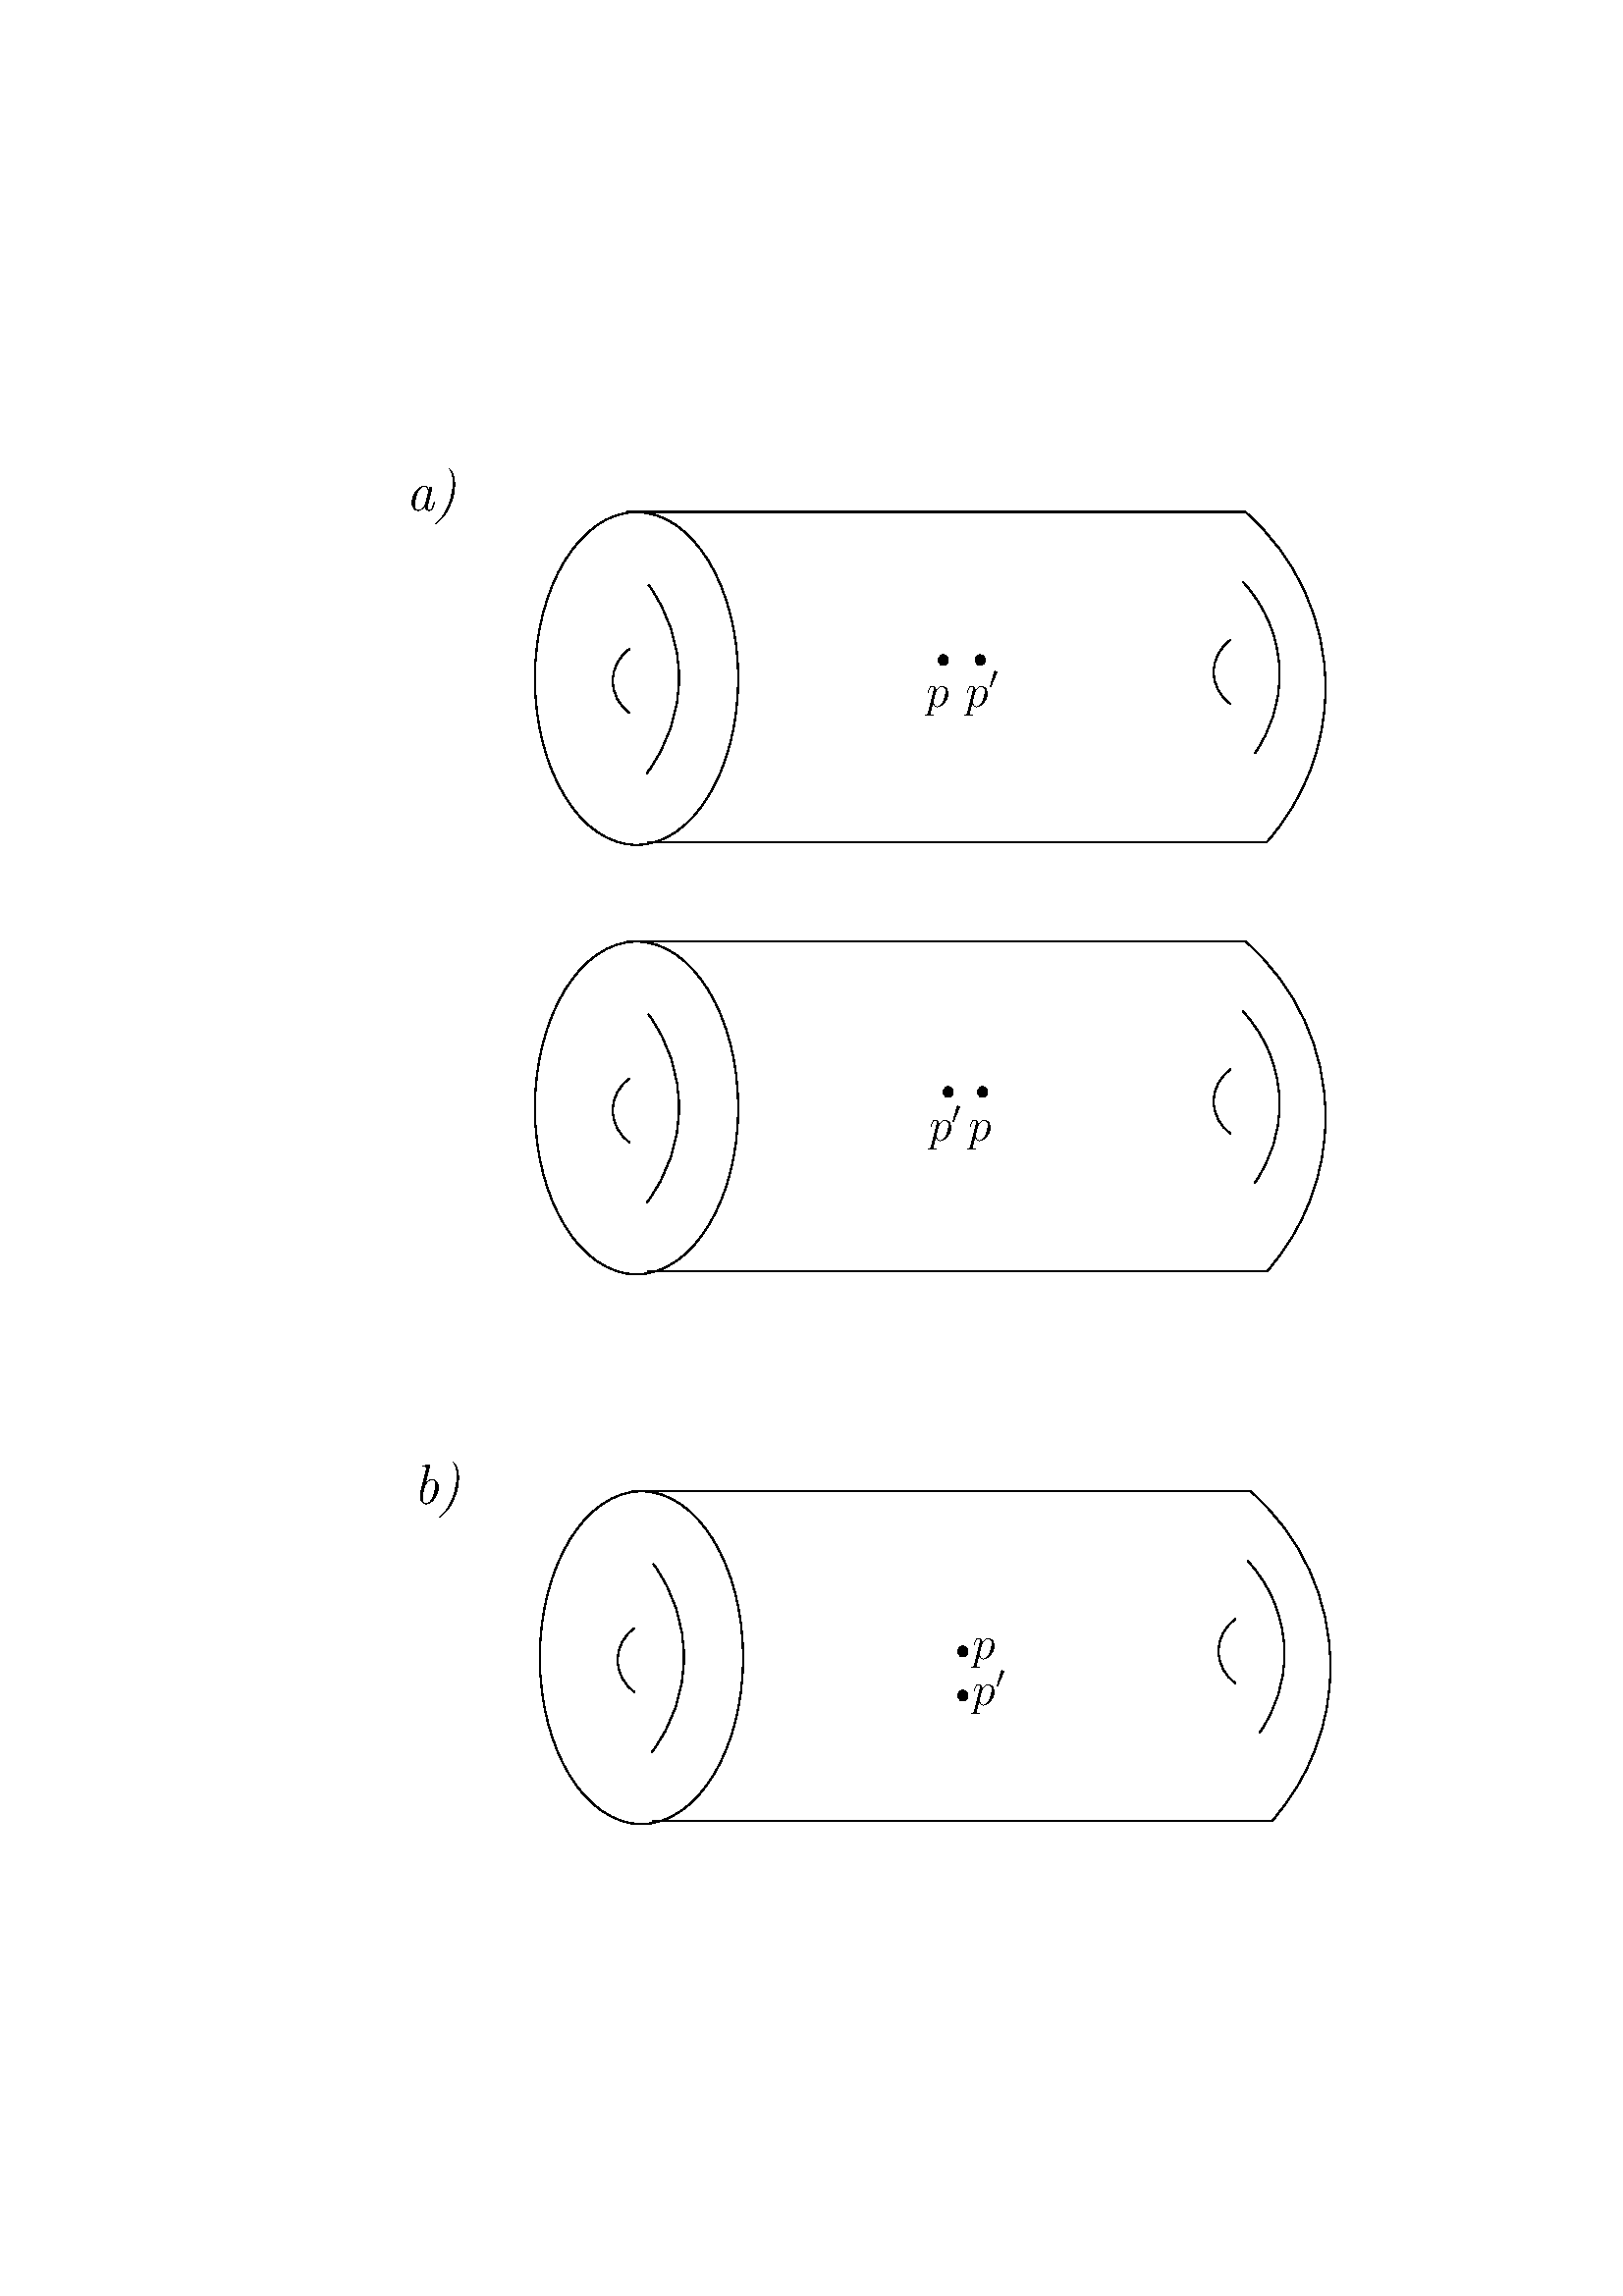
\includegraphics[width=0.75\linewidth]{figures/gla7-7.png}
\caption{(a) Two partial resolutions of singularity. The moduli space is a fiber bundle parameterizing successive Hecke modifications at the same point $z\in C$. (b) A partial deformation of singularity. The moduli space is a product, parameterizing independent Hecke modifications at distinct points $z,z'\in C$.（原文 Fig.~18）}
\label{fig:xdtampo}
\end{figure}

What is the space $\bar\EUZ{}^*$ that has the simultaneous
deformations and resolutions just described? It is in fact
$\bar{\EUZ}(^L\bar w,p')$, the compactified moduli space of
solutions of the Bogomolny equations in the presence of a single
't Hooft operator of weight $^L\bar w={}^L\negthinspace
w+{}^L\negthinspace w'$.

{}From a physical point of view, this statement is part of the
operator product expansion of the operators $T(^L\negthinspace
w,p)$ and $T(^L\negthinspace w',p')$. We discussed some general
properties of this expansion in section 第~\ref{sec:lineop}~节. Simple arguments
that we explained there suffice to show that the product
$T(^L\negthinspace w,p)\cdot T(^L\negthinspace w',p')$ has an
expansion as $\sum_{i\in \EUR}c_i T(^L\negthinspace w_i,p')$, for
some set $\EUR$ of weights $^L\negthinspace w_i$ and coefficients
$c_i$. $S$-duality predicts the detailed form of this expansion
(which should match the representation ring of $^L\negthinspace
G$), but it is difficult to verify this prediction directly.
However, the simple arguments of section 第~\ref{sec:lineop}~节\ do suffice to
show that the form of the expansion as $p\to p'$ is
% 式 (10.20)
\setcounter{equation}{19}
\begin{equation}\label{eq:hittor}
T({}^L\negthinspace w,p)\cdot T({}^L\negthinspace
w,p')\to T({}^L\bar w,p')+\sum_{i\in \EUR'} c_i
T({}^L\negthinspace w_i,p'),
\end{equation}
 where $^L\bar w={}^L\negthinspace
w+{}^L\negthinspace w'$, and the weights $^L\negthinspace
w_i,\,i\in \EUR'$ are the dominant weights such that $^L\bar
w-{}^L\negthinspace w_i$ is also dominant. This means that
$^L\negthinspace w_i$ is what we have called an associated weight
of $^L\bar w$.

The formula \eqref{eq:xinon}\ shows that the dimension of $\bar\EUZ(^L\bar
w,p')$ precisely equals the dimension of $\bar\EUZ(^L\negthinspace
w,p;{}^L\negthinspace w',p')$. This is consistent with the
statement that the former is the limit of the latter for $p\to
p'$.  Other spaces $\bar\EUZ(^L\negthinspace w_i,p')$, $i\in
\EUR'$ have strictly smaller dimension. In fact, in a certain
sense, the spaces $\bar\EUZ(^L\negthinspace w_i,p')$ all appear in
the limit of $\bar\EUZ(^L\negthinspace w,p;{}^L\negthinspace
w',p')$ for $p\to p'$. Since the $^L\negthinspace w_i$ are
associated weights of $^L\bar w_i$, the natural compactification
$\bar {{\EUY}}(^L\bar w)$ of the space of Hecke modifications of
type $^L\bar w$ includes the spaces $\bar {{\EUY}}(^L\negthinspace
w_i)$  of Hecke modifications of types $^L\negthinspace w_i$, for
all $i\in \EUR'$.  In terms of Bogomolny moduli spaces, this means
that the spaces $\bar\EUZ(^L\negthinspace w_i,p')$ are all
contained in the singular ``monopole bubbling'' locus of
$\bar\EUZ(^L\bar w,p')$.

This is why it is difficult to determine the operator product
expansion for 't Hooft operators; the subleading terms in \eqref{eq:hittor}\
all come entirely from singularities of $\bar\EUZ(^L\bar w,p')$.
In section 第~\ref{sec:opprod}~节, we will explain certain mathematical results
\cite{ref97,ref98} which from a
physical point of view are equivalent to determining the full
operator product expansion.

First, however, we want to recall an example analyzed in section
第~\ref{sec:spaceheck}~节\ that provides a good illustration of these arguments.
Take $G=PSU(2)$, $\LG=SU(2)$, $^L\negthinspace w={}^L\negthinspace
w'=(1/2,-1/2),$ and $^L\bar w={}^L\negthinspace
w+{}^L\negthinspace w'=(1,-1)$. The weights $^L\negthinspace w$
and $^L\bar w$ correspond to the two-dimensional and the adjoint
representations of $\LG=SU(2)$, respectively. As we learned in
section 第~\ref{sec:spaceheck}~节, the  spaces $\bar {{\EUZ}}(^L\negthinspace
w,z)$ and $\bar {{\EUZ}}(^L\negthinspace w',z)$ are copies of
$\Bbb{CP}^1$. The space $\bar\EUZ{}^*=\bar {{\EUZ}}(^L\bar w,z)$
is the weighted projective plane $\Bbb{WCP}^2(1,1,2)$ and has an
orbifold singularity. We have found that this singular space can
be deformed into a product $\Bbb{CP}^1\times\Bbb{CP}^1$ and also
resolved into a Hirzebruch surface which is a $\Bbb{CP}^1$ bundle
over $\Bbb{CP}^1$. We also saw that the resolution and deformation
are compatible, in the sense that the Hirzebruch surface can be
deformed into $\Bbb{CP}^1\times\Bbb{CP}^1$. All this is in accord
with the above general arguments.  (However, in this particular
example, $^L\negthinspace w={}^L\negthinspace w'$, so the two
resolutions are equivalent.)

In this example, there is a unique way to write $^L\bar w$ as a
sum of nonzero positive weights.  In general, there will be
several ways to do this and thus several choices of partial
resolutions and desingularizations of $\bar {{\EUZ}}(^L\bar w,z)$
along these lines.  For a simple Lie group $^L\negthinspace G$ of
rank $r$, there are $r$ fundamental weights $^L\negthinspace
w_\gamma$, $\gamma=1,\dots,r$, such that any dominant weight
$^L\bar w$ can be uniquely expanded $^L\bar
w=\sum_{\gamma=1}^r t_\gamma {}^L\negthinspace w_\gamma$ with some
non-negative integers $t_\gamma$.  (For example, if
$^L\negthinspace G=SU(r+1)$, the $^L\negthinspace w_\gamma$ are
the highest weights of the minuscule representations
$\wedge^\gamma \VV$, $\gamma=1,\dots r$. These are called the
fundamental representations.) The maximum partial resolution and
desingularization of $\bar {{\EUY}}(^L\bar w,z)$ that we can make
using the Bogomolny equations is to relate it to a moduli space
with $t_\gamma$ insertions of 't Hooft operators of type
$^L\negthinspace w_\gamma$, for $\gamma=1,\dots,r$.  For
$SU(r+1)$, since the fundamental representations  are minuscule,
this gives a complete resolution or deformation of singularities
of the space of Hecke modifications of any given weight.

For other groups, the best we can do is to reduce to the
singularities of a product of 't Hooft operators
$T({}^L\negthinspace w_\gamma)$ with fundamental weights.  The
space of Hecke modifications for such an operator has
singularities, associated with monopole bubbling, that can be
locally modeled by a hyper-Kahler manifold, but there is no
obvious hyper-Kahler resolution of these singularities.
